\documentclass[a4paper, 11pt]{book}
\usepackage{graphicx}
\title{Python for the Under 10's}
\author{Graeme Winter}
\begin{document}
\maketitle
\clearpage
\chapter{Introduction}

\section{Preface for Grown Ups}

When the author was a child computers were smaller, simpler and harder to break\footnote{Machines like the BBC Model B, ZX81 and Spectrum 48k spring to mind}, and so much more suitable for leaning how they work. Today computers are bigger, more complex, easier to break and much less straightforward to understand. At the same time they are used for everything: from catching up on TV to reading the news, communicating with people and gaming. This has meant that the creative process of writing simple computer programs (typically games) has been lost in favour of easily accessed entertainment. While none of this is a bad thing, it has removed the opportunity to learn \emph{how they work}. The idea of this book is to provide this opportunity, using free tools and real programming languages. 

The pre-requisite for this is a relatively recent computer - anything bought since about 2005 or so, running Windows, Linux or Mac OS X should be fine. The only dependency is the installation of Python 2.7.3 or later from http://www.python.org. If you have an old laptop lying around which used to be useful and is no longer, this will probably be fine. 

\section{Preface for Children}

Most grown ups use computers for a lot of the day, but most of them have no idea how they work - the idea of this book is to help you learn how they work and what they can do. Telling the computer what to do is called programming, and there are lots of different languages you can use to tell the computer wha to do. This book is about one called Python (yes, like the snake) which is god because it is one of the easiest and also lets you do fun things straight away.

Some people say programming is hard, and sometimes it is, but the hardest bit is thinking about what you want the computer to do in little pieces - once you have done this getting the computer to do the work is easy. That's enough - let's get started!

\section{Getting Started}

The only thing that is needed is to install Python - which you can download from http://www.python.org. This is free but it is probably better if a grown up installs it. To use it you will need to do some typing in something called a terminal - on an Apple computer they look like this:

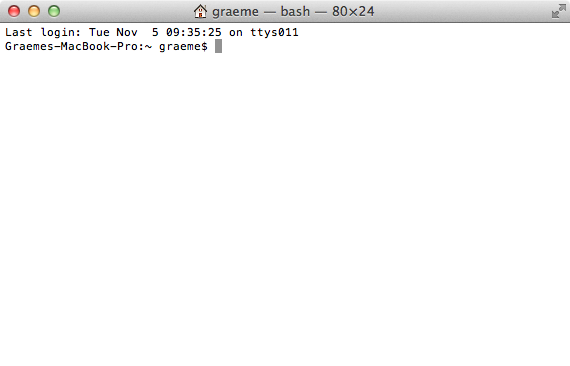
\includegraphics[scale=0.4]{terminal.png}

\noindent
and they let you talk to the computer. All you need to do in here is type ``python'' and you should see

{\small
\begin{verbatim}
Python 2.7.3 (default_cci, Dec 13 2012, 05:32:36) 
[GCC 4.2.1 (Apple Inc. build 5666) (dot 3)] on darwin
Type "help", "copyright", "credits" or "license" for more information.
>>> 
\end{verbatim}
}

\noindent 
or something similar which says that the computer is ready to start talking to you in Python. If you see this then everything is set up just fine.

\chapter{Pythons and Turtles}

\end{document}